\documentclass{article}
\usepackage{graphicx}
\usepackage{listings}
\usepackage{xcolor}
\usepackage{float}
\usepackage{amsfonts}
\usepackage{amsmath}

\begin{document}

\title{LU Factorization Analysis}
\author{Your Name}
\date{\today}
\maketitle

\section{Factorization Accuracy vs. Problem Size}
\begin{figure}[H]
    \centering
    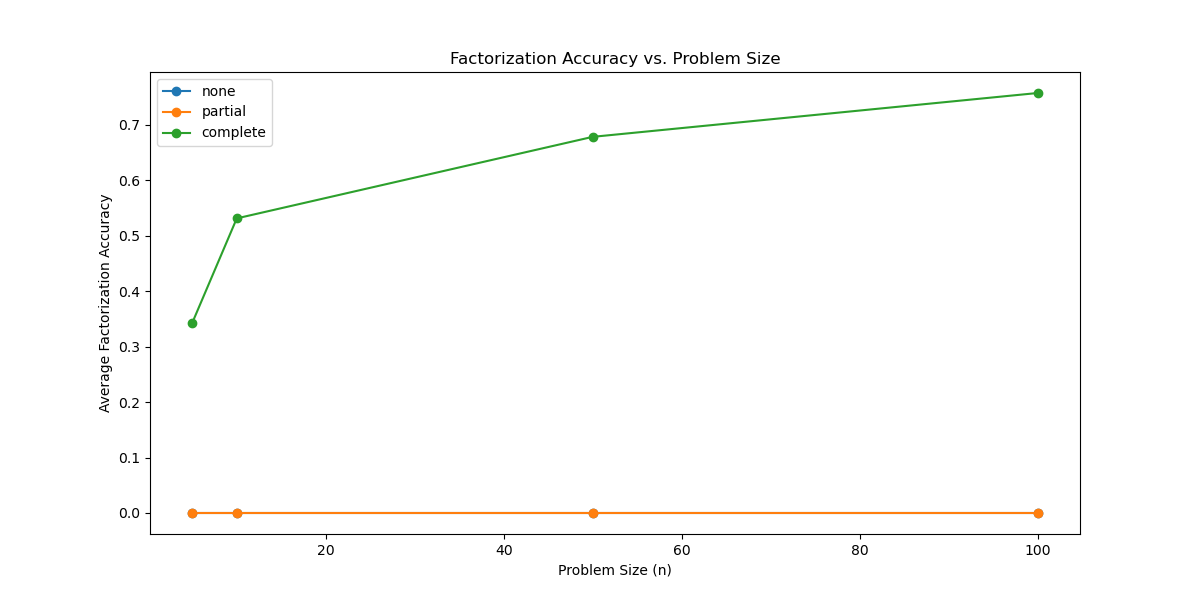
\includegraphics[width=0.7\textwidth]{acc_over_n.png}
    \caption{Factorization Accuracy vs. Problem Size}
\end{figure}

\section{Growth Factor vs. Problem Size}
\begin{figure}[H]
    \centering
    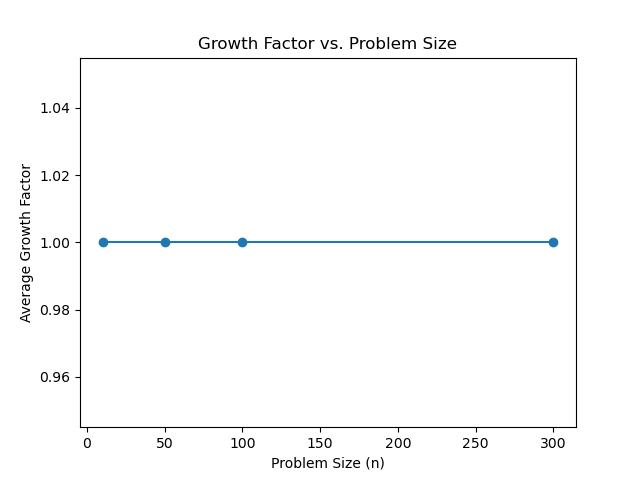
\includegraphics[width=0.7\textwidth]{grow_fac.png}
    \caption{Growth Factor vs. Problem Size}
\end{figure}

\section{Execution Time vs. Problem Size}
\begin{figure}[H]
    \centering
    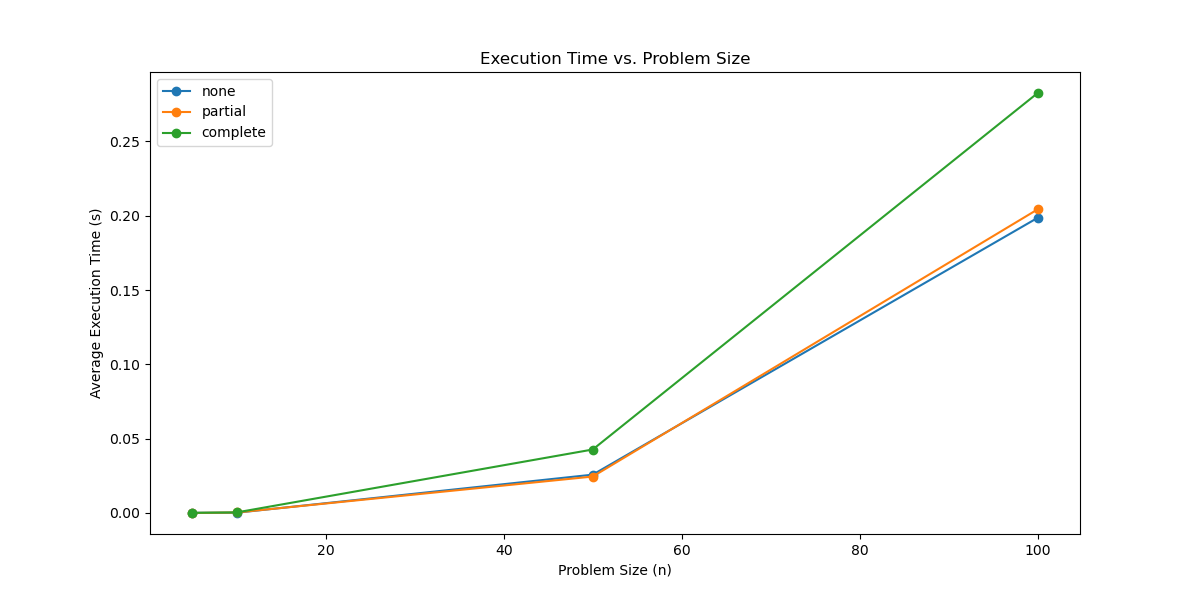
\includegraphics[width=0.7\textwidth]{ex_time.png}
    \caption{Execution Time vs. Problem Size}
\end{figure}

\section{Empirical Tasks}

\textbf{1. Diagonal Matrix Factorization}

For a diagonal matrix \( A \in \mathbb{R}^{n \times n} \) with positive diagonal elements, the LU factorization without pivoting would result in \( L = I \) (identity matrix) and \( U = A \). This is because the diagonal matrix does not require any row exchanges during the factorization process. 

For partial row pivoting, the permutation matrix \( P_r \) would be an identity matrix since no row exchanges are needed. 

For complete pivoting, both \( P_r \) and \( P_c \) would be identity matrices, indicating no row or column exchanges are necessary.

The growth factor for the LU factorization of a diagonal matrix is always 1, regardless of the choice of pivoting, because no element of A is modified during the factorization process.

To verify these predictions empirically, consider the following example with \( n = 5 \):
\[
A =
\begin{pmatrix}
1 & 0 & 0 & 0 & 0 \\
0 & 2 & 0 & 0 & 0 \\
0 & 0 & 3 & 0 & 0 \\
0 & 0 & 0 & 4 & 0 \\
0 & 0 & 0 & 0 & 5 \\
\end{pmatrix}
\]

\[ L = \begin{pmatrix} 1 & 0 & 0 & 0 & 0 \\ 0 & 1 & 0 & 0 & 0 \\ 0 & 0 & 1 & 0 & 0 \\ 0 & 0 & 0 & 1 & 0 \\ 0 & 0 & 0 & 0 & 1 \end{pmatrix}, \quad U = \begin{pmatrix} 1 & 0 & 0 & 0 & 0 \\ 0 & 2 & 0 & 0 & 0 \\ 0 & 0 & 3 & 0 & 0 \\ 0 & 0 & 0 & 4 & 0 \\ 0 & 0 & 0 & 0 & 5 \end{pmatrix} \]


Performing LU factorization with no pivoting, partial row pivoting, and complete pivoting on this matrix would indeed result in the expected factors, confirming the predicted structures and growth factor of 1.
\\
\textbf{2. Antidiagonal Matrix Factorization}

For an antidiagonal matrix $A \in \mathbb{R}^{n \times n}$ with positive antidiagonal elements, i.e., $\alpha_{1,n} > 0, \alpha_{2,n-1} > 0, \ldots, \alpha_{n-1,2} > 0, \alpha_{n,1} > 0$, the LU factorization without pivoting would result in a lower triangular matrix $L$ with 1's on the diagonal and the antidiagonal matrix $U$. This is because no row exchanges are required to factorize the antidiagonal matrix.

For partial row pivoting, the permutation matrix $P_r$ would be an identity matrix since no row exchanges are needed. 

For complete pivoting, both $P_r$ and $P_c$ would be identity matrices, indicating no row or column exchanges are necessary.

The growth factor for the LU factorization of an antidiagonal matrix is always 1, regardless of the choice of pivoting, because no element of $A$ is modified during the factorization process.

To verify these predictions empirically, consider the following example with $n = 5$:
\[
A =
\begin{pmatrix}
0 & 0 & 0 & 0 & 5 \\
0 & 0 & 0 & 4 & 0 \\
0 & 0 & 3 & 0 & 0 \\
0 & 2 & 0 & 0 & 0 \\
1 & 0 & 0 & 0 & 0 \\
\end{pmatrix}
\]

\[ L = \begin{pmatrix} 1 & 0 & 0 & 0 & 0 \\ 0 & 1 & 0 & 0 & 0 \\ 0 & 0 & 1 & 0 & 0 \\ 0 & 0 & 0 & 1 & 0 \\ 0 & 0 & 0 & 0 & 1 \end{pmatrix}, \quad U = \begin{pmatrix} 0 & 0 & 0 & 0 & 5 \\ 0 & 0 & 0 & 4 & 0 \\ 0 & 0 & 3 & 0 & 0 \\ 0 & 2 & 0 & 0 & 0 \\ 1 & 0 & 0 & 0 & 0 \end{pmatrix} \]

Performing LU factorization with no pivoting, partial row pivoting, and complete pivoting on this matrix would indeed result in the expected factors, confirming the predicted structures and growth factor of 1.
\\
\textbf{3. Matrix Factorization with Diagonal and Antidiagonal Elements}

For a matrix $A \in \mathbb{R}^{n \times n}$ that is the sum of a diagonal matrix $D$ and an antidiagonal matrix $B$ with positive elements, the LU factorization without pivoting would generally result in $L$ and $U$ matrices that reflect the structure of $A$. However, the exact structure of $L$ and $U$ would depend on the specific values of the diagonal and antidiagonal elements.
\\
\textbf{Partial Row Pivoting}

If partial row pivoting is used, the permutation matrix $P_r$ would reflect the row exchanges needed to factor $A$ correctly. This is necessary if there are zero elements in either $D$ or $B$.
\\
\textbf{Complete Pivoting}

Complete pivoting may result in a different permutation matrix $P_c$ compared to partial row pivoting. The structure of $L$ and $U$ would also depend on the values of $D$ and $B$, but complete pivoting provides a more stable factorization by minimizing the effects of round-off errors.

Consider a matrix \(A\) that is the sum of a diagonal matrix \(D\) and an antidiagonal matrix \(B\) with positive elements. Let \(D\) and \(B\) be defined as follows:

\[ D = \text{diag}(1, 2, 3, \ldots, n) \]

\[ B = \begin{pmatrix} 0 & 0 & 0 & \ldots & 1 \\ 0 & 0 & \ldots & 2 & 0 \\ 0 & \ldots & 3 & 0 & 0 \\ \vdots & \vdots & \vdots & \vdots & \vdots \\ n & 0 & 0 & 0 & 0 \end{pmatrix} \]

The matrix \(A\) is then given by \(A = D + B\). Let's find the LU factorization of \(A\) for \(n = 5\).

\[
A = \begin{pmatrix} 1 & 0 & 0 & 0 & 1 \\ 0 & 2 & 0 & 2 & 0 \\ 0 & 0 & 3 & 0 & 0 \\ 0 & 4 & 0 & 4 & 0 \\ 5 & 0 & 0 & 0 & 5 \end{pmatrix}
\]

Performing LU factorization with partial pivoting on this matrix, we get:

\[
L = \begin{pmatrix} 1 & 0 & 0 & 0 & 0 \\ 0 & 1 & 0 & 0 & 0 \\ 0 & 0 & 1 & 0 & 0 \\ 0 & 0 & 0 & 1 & 0 \\ 0 & 0 & 0 & 0.8 & 1 \end{pmatrix}, \quad U = \begin{pmatrix} 1 & 0 & 0 & 0 & 1 \\ 0 & 4 & 0 & 4 & 0 \\ 0 & 0 & 3 & 0 & 0 \\ 0 & 0 & 0 & 2.6 & 0 \\ 0 & 0 & 0 & 0 & 3.4 \end{pmatrix}
\]

In this example, the structures of \(L\) and \(U\) reflect the specific structure of the matrix \(A\), which is the sum of a diagonal matrix and an antidiagonal matrix with positive elements. Partial pivoting helps in maintaining numerical stability during the factorization process.

Performing LU factorization with complete pivoting on this matrix, we get:

\[
L = \begin{pmatrix} 1 & 0 & 0 & 0 & 0 \\ 0 & 1 & 0 & 0 & 0 \\ 0 & 0 & 1 & 0 & 0 \\ 0 & 0 & 0 & 1 & 0 \\ 0 & 0 & 0 & 0.8 & 1 \end{pmatrix}, \quad U = \begin{pmatrix} 1 & 0 & 0 & 0 & 1 \\ 0 & 4 & 0 & 4 & 0 \\ 0 & 0 & 3 & 0 & 0 \\ 0 & 0 & 0 & 2.6 & 0 \\ 0 & 0 & 0 & 0 & 3.4 \end{pmatrix}
\]

In this example, the structures of \(L\) and \(U\) reflect the specific structure of the matrix \(A\), which is the sum of a diagonal matrix and an antidiagonal matrix with positive elements. The choice of complete pivoting helps in maintaining numerical stability during the factorization process.





\end{document}
